\documentclass[11pt,a4paper]{article}
\usepackage[T1]{fontenc}
\usepackage{graphicx}
\usepackage{mathtools}
\usepackage{amssymb}
\usepackage{geometry}
\usepackage{titlesec}
\usepackage{enumitem} % 添加enumitem宏包
\usepackage{amsfonts}
\usepackage{amssymb}
\usepackage{fancyhdr} % 添加fancyhdr宏包
\usepackage{lastpage} % 添加lastpage宏包
\usepackage{graphicx} % 导入graphicx包
\usepackage{gensymb} % 引入gensymb包
\usepackage[UTF8]{ctex}
% 应用fancyhdr宏包的页脚样式
\pagestyle{fancy}
\fancyhf{} % 清除当前的页眉页脚设置
\fancyfoot[L]{免费开源,请勿商用} % 页脚左下方显示文字
\fancyfoot[R]{作者:阿尧} % 页脚右下方显示文字
\renewcommand{\headrulewidth}{0pt} % 去掉页眉的横线
\renewcommand{\footrulewidth}{1pt} % 设置页脚的横线宽度
\usepackage{draftwatermark} %增加水印
\SetWatermarkText{本真题由b站up陈瀚尧探索世界免费开源}
\SetWatermarkScale{0.3} % 可以调整为合适的大小
\SetWatermarkColor{gray!50} % 灰色透明度为50%

% 设置更窄的页面边距
\geometry{left=3cm, right=3cm, top=1cm, bottom=2cm}

% 设置section标题格式
\titleformat{\title}{\bfseries}{\thetitle}{1em}{}

% 设置section之间的距离
\titlespacing*{\section}{0pt}{3.25ex plus 1ex minus .2ex}{1.5ex plus .2ex}

\begin{document}
    \title{中国科学院大学\\2017年招收攻读硕士学位研究生入学统一考试试题\\科目名称:光学}
    \author{制作者:b站up 陈瀚尧探索世界}
    \date{}
    \maketitle
    % 设置section标题不显示序号
    \titleformat{\section}[block]{\normalfont\Large\bfseries}{}{0pt}{}

    % 设置itemize环境的项目符号为空
    \setlist[itemize]{label=} 

    \section{考试须知:}
    \begin{itemize}[topsep=0pt,itemsep=0pt,partopsep=0pt]
        \item 1.本试卷满分为150分,全部考试时间总计180分钟。
        \vspace{-3mm}
        \item 2.所有答案必须写在答题纸上,写在试题纸上或草稿纸上一律无效。
        \vspace{-3mm}
        \item 3.可以使用无字典存储或编程功能的电子计算器。(此条对于25考研可能作废)
    \end{itemize}
    \vspace{-5mm}
    \noindent\rule{\textwidth}{0.5pt} % 添加一条线
    \vspace{-12mm}
    \section*{一、名词解释(16分,每小题4分)}
    \begin{enumerate}
        \vspace{0mm}
        \item 辐射通量、辐照度
        \vspace{15mm}
        \item 球差、位置色差
        \vspace{15mm}
        \item 孔径光阑、视场光阑
        \vspace{15mm}
        \item 主点、节点
        \vspace{15mm}
    \end{enumerate}
    \subsection*{2.如图所示,双球面反射镜系统由主镜和次镜构成。主镜顶点为A,次镜顶点为B,主镜曲率半径为$r_1$,次镜曲率半径为$r_2$,F为系统像方焦点,系统总焦距$f^{'}=500mm$。若要求将无限远目标成像在$F^{'}$处,$F^{'}$位于A点后方20mm,且次镜的垂轴放大率$\beta _{2}=-5^{x}$,试求$r_1$,$r_2$和主次镜的间隔$|AB|$。}
    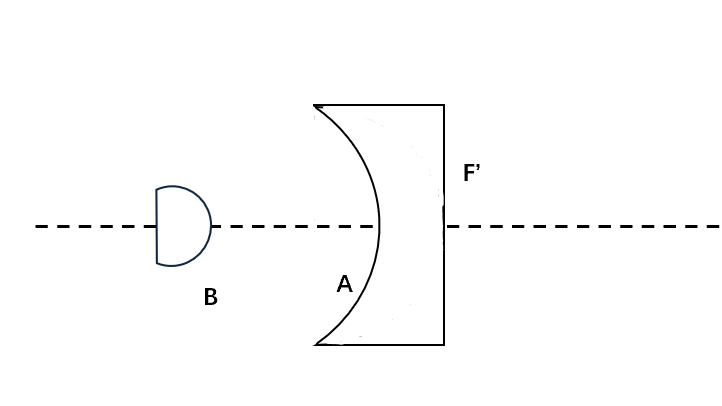
\includegraphics[scale=0.2]{1.png}% 插入图片,按50%的比例缩放
    \vspace{10mm}
    \subsection*{3.位于空气中的两个薄透镜(即每一个透镜本身的两主面重合),其参数分别为$f_1^{'}=90mm$,$f_2^{'}=60mm$,间隔$d=40mm$}
    \begin{itemize}
        \vspace{0mm}
        \item (1)求组合系统的焦距;
        \vspace{0mm}
        \item (2)求物方焦点和物方主点的位置;
        \vspace{0mm}
        \item (3)求像方焦点和像方主点的位置。
        
        %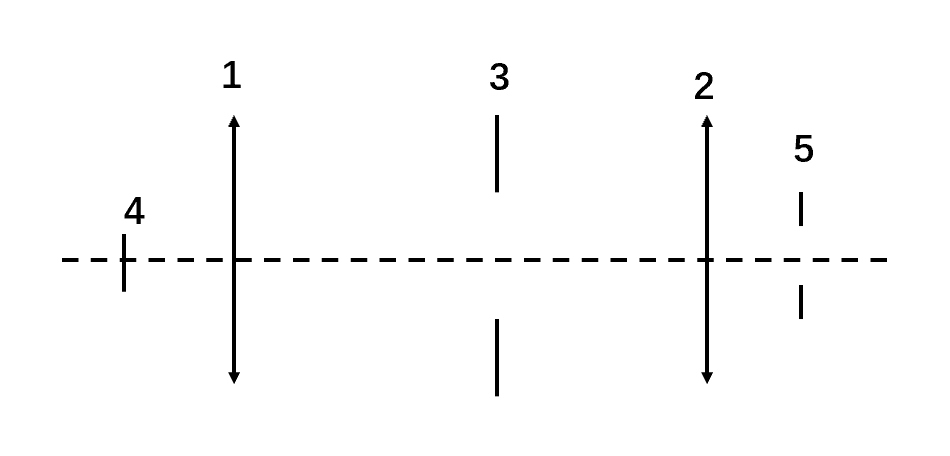
\includegraphics[scale=0.2]{2.png}% 插入图片,按50%的比例缩放
    \end{itemize}
    \vspace{20mm}
    \subsection*{4.如图所示为焦距仪读数显微镜的光学系统,1为物镜,2为目镜,3为分化板,4为物,5为出窗。已知物体$2y=10mm$,物镜放大倍率$\beta =-1^{x}$,$tgU=0.1$($U$为物镜的半孔径角),物体位于空气中,物距$l$为130mm,分化板到目镜的距离为20mm,目镜焦距$f_{11}^{'}$为20mm,物镜框是孔径光阑,分化板为视场光阑。试求:}
    \begin{itemize}
        \vspace{0mm}
        \item (1)物镜焦距;
        \vspace{0mm}
        \item (2)整个光学系统的入瞳、出瞳位置和大小;
        \vspace{0mm}
        \item (3)整个光学系统物方视场角$2\omega $和像方视场角为$2\omega^{'}$;
        \vspace{0mm}
        \item (4)物面无渐晕条件下目镜的通光孔径。
        
        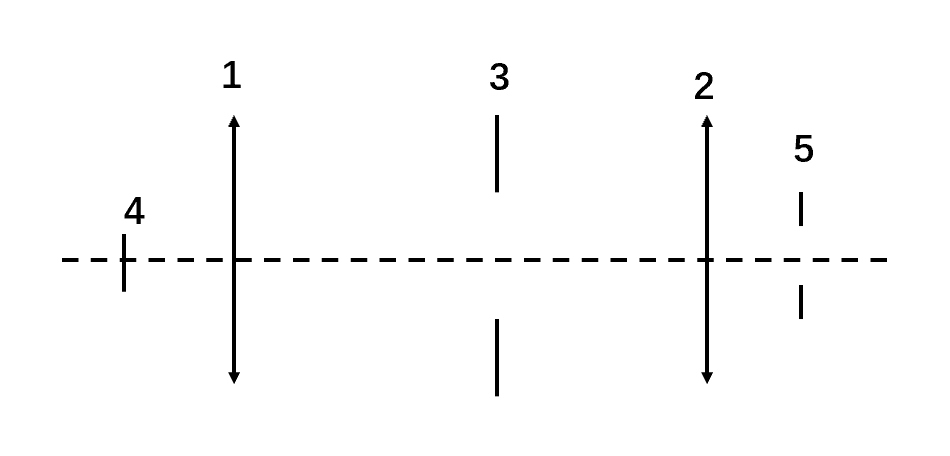
\includegraphics[scale=0.2]{2.png}% 插入图片,按50%的比例缩放
    \end{itemize}
    \vspace{20mm}
    \subsection*{5.试确定光波场$E_x=E_0\sin(\omega t-kz)$、$E_y=E_0\cos (\omega t-kz+\frac{\pi}{4})$的偏振状态,并写出其归一化琼斯矢量形式。}
    \vspace{10mm}
    \subsection*{6.一左旋圆偏振光,以$60\degree $角由玻璃斜入射到空气界面上,玻璃和空气的折射率分别为1.5和1。试确定界面反射光的偏振状态。}
    \vspace{10mm}
    \subsection*{7.在杨氏双缝干涉实验装置中,双缝相距0.5mm,接收屏距双缝1m,点光源距双缝30cm,发射$\lambda =500nm$的单色光。试求:}
    \begin{itemize}
        \vspace{0mm}
        \item (1)屏上干涉亮条纹位置。
        \vspace{0mm}
        \item (2)若点光源由轴上向下平移2mm,接收屏上干涉条纹向什么方向移动?移动多少距离?
        \vspace{0mm}
        \item (3)若光源由点光源变为具有一定的宽度,并且恰恰使得接收屏上的干涉条纹消失,该宽度是多少?
        
        %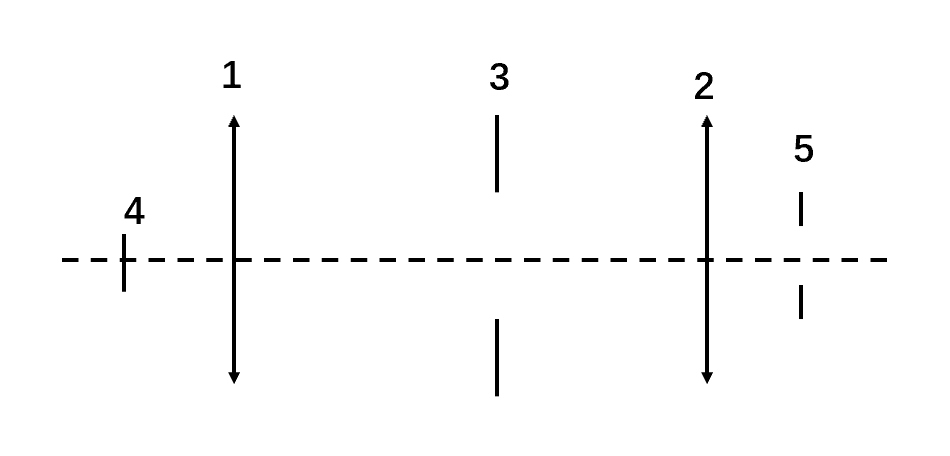
\includegraphics[scale=0.2]{2.png}% 插入图片,按50%的比例缩放
    \end{itemize}
    \vspace{20mm}
    \subsection*{8.图示双光束干涉实验,一波长$\lambda =10\mu m$、相干长度$l_c=5\lambda$的细光束,以$60\degree$角入射到厚度$h=10\mu m$、折射率$n_1=\sqrt{3}$的介质片1上,由其上表面反射的光束经厚度为d、折射率$n_2=1.5$的介质片2后,被透镜聚焦在$P_0$点与来自介质片1下表面的反射光干涉。若$P_0$点恰为亮点,求介质片2的厚度d为多大?}

    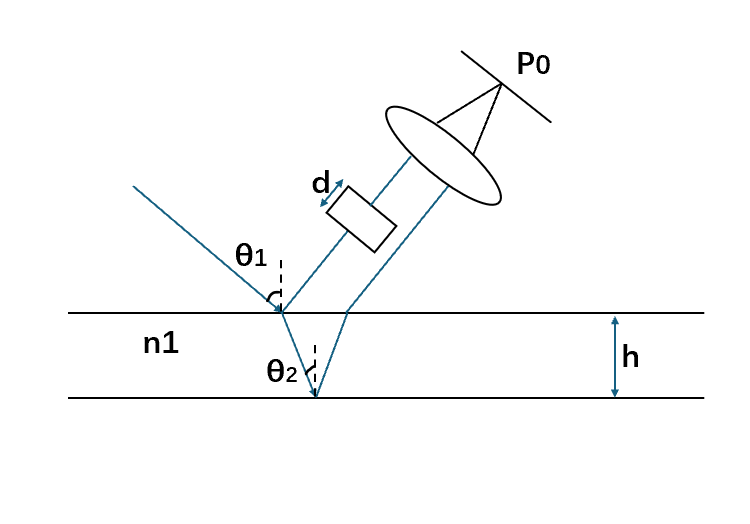
\includegraphics[scale=0.2]{3.png}% 插入图片,按50%的比例缩放
    \vspace{20mm}
    \subsection*{9.一台显微镜的数值孔径为0.9}
    \begin{itemize}
        \vspace{0mm}
        \item (1)试求550nm光照明时的最小分辨距离。
        \vspace{0mm}
        \item (2)当用波长为400nm的紫色光照明时,它的分辨本领相对(1)提高多少倍?
        \vspace{0mm}
        \item (3)在(2)的条件下,进而采用油浸系统($n=1.6$)时,最小分辨距离是多少?
    \end{itemize}
    \vspace{10mm}
    \subsection*{10.一块闪耀光栅宽260mm,每毫米内有300个刻槽,闪耀角为$77\degree12^{'}$。}
    \begin{itemize}
        \vspace{0mm}
        \item (1)求光束垂直槽面入射时,对于波长$\lambda =500nm$光的分辨本领;
        \vspace{0mm}
        \item (2)光栅的自由光谱范围有多大?
    \end{itemize}
    \vspace{10mm}
    \subsection*{11.图示方解石棱镜的主折射率为$n_o=1.6408$,$n_e=1.4790$,}
    \begin{itemize}
        \vspace{0mm}
        \item (1)若要使其成为格兰-傅科棱镜工作,其直角棱镜底角$\theta$应选为多大?
        \vspace{0mm}
        \item (2)试绘出自然光正入射时的传输光路及光的偏振状态。
    \end{itemize}
    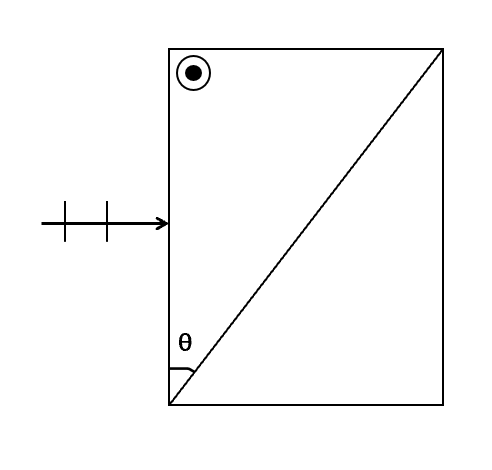
\includegraphics[scale=0.2]{4.png}% 插入图片,按50%的比例缩放
    \vspace{10mm}
    \subsection*{12.一厚度为0.04mm的方解石晶片($n_o=1.6548$,$n_e=1.4864$,不计色散),光轴平行于表面,插在两个正交偏振片之间,且其主截面与起偏器偏振方向成$\theta$角度($\theta\neq 0\degree,90\degree$)。试确定632.8nm红光能否透过该装置。}
    \vspace{10mm}
\end{document}